% !TeX root = ../thesis.tex

\chapter{随机传值进程模型的应用}

Random VPC可以用于对云计算协议的形式刻画。
在此我们对一种云计算协议:Gossip-Style Membership Protocol进行建模和模拟实现。

\section{Gossip Style Membership协议}
\subsection{Gossip协议}
Gossip协议分为push gossip和pull gossip两种。
\begin{itemize}
   \item {
      \textbf{Push Gossip:} 
      
      消息的发送者周期性的随机选择$k$个目标节点发送Gossip Message。
      接收到Gossip Message的节点可以根据本地时间,周期性的选择$b$个目标节点发送Gossip Message。
      在发送过程中,已经拥有Gossip Message的节点仍然可以被选为目标节点。
   }
   \item {
      \textbf{Pull Gossip:}

      每个节点周期性的向$k$个目标节点发送Gossip Query,
      收到Gossip Query的节点若拥有Gossip Message的节点会向发送Query的节点返回Gossip Message的拷贝。
   }
\end{itemize}

在超过$\frac{n}{2}$的节点拥有Gossip Message时,可以证明此时选择Pull Gossip会比Push Gossip传播的更快[此处应有引用]。
因此在使用Gossip协议时,常使用Push Gossip与Pull Gossip的混合:
在消息传播$\frac{n}{2}$节点之前使用Push Gossip,在消息传播$\frac{n}{2}$之后使用Pull Gossip。

\subsection{Gossip Style Membership协议}

在数据中心中会频繁的出现节点的失效,
我们会为每一个节点维护一个Membership List来记录数据中心中其他节点的运行情况。
Membership Protocol是一个通过网络检测节点失效和传播失效信息的机制,
常用的Membership Protocol有Heartbeating Protocol, Gossip-Style Membership Protocol, SWIM Failure Detector Protocol等。

Gossip-Style Membership Protocol使用Gossip协议传递每个节点的Membership List。
每个节点周期性的随机选择$k$个节点发送自己的Membership List,
收到Membership List的节点根据其他节点的Membership List更新自己的Membership List。

\section{Gossip Style Membership的实现}
\subsection{Push Gossip协议的实现}
由于Push Gossip实现难度较小,并且单一的Push Gossip协议仍然可以达到$O(\log N)$时间复杂度的消息传播,
我们以Push Gossip协议的实现作为Random VPC的demo。
其中Gossip单节点的通道示意图如图1。
以Gossip协议作为通信协议的四节点的Peer-to-Peer Sysyem的示意图如图2。

\begin{figure}[!htbp]
	\small
	\centering
	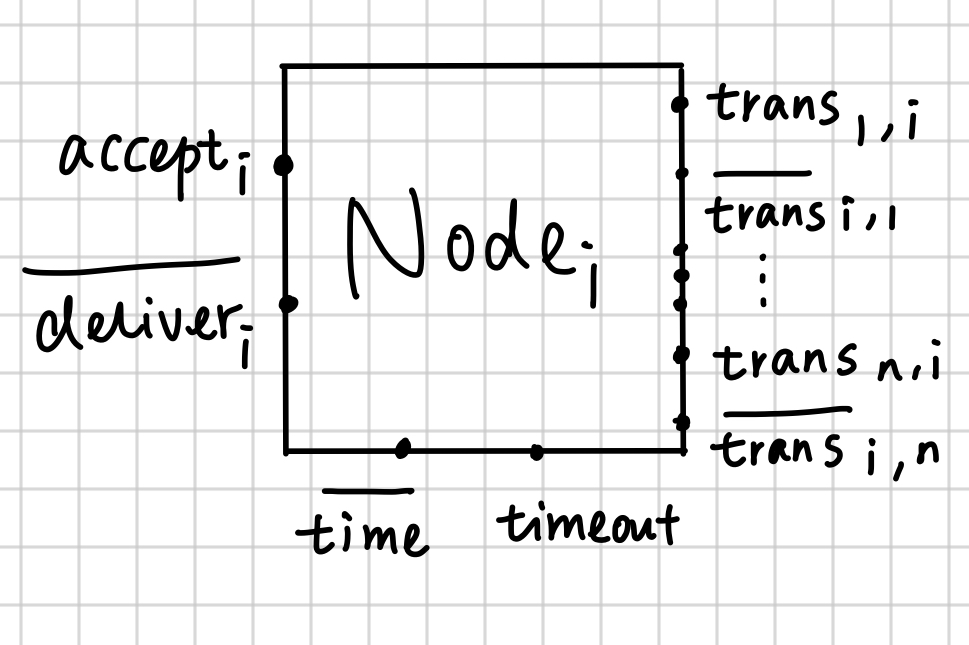
\includegraphics[width=6cm]{../figure/gossip1.jpg}
    \caption{\textbf{Gossip 节点示意图}}
    \label{fig1}
\end{figure}

\begin{figure}[!htbp]
	\small
	\centering
	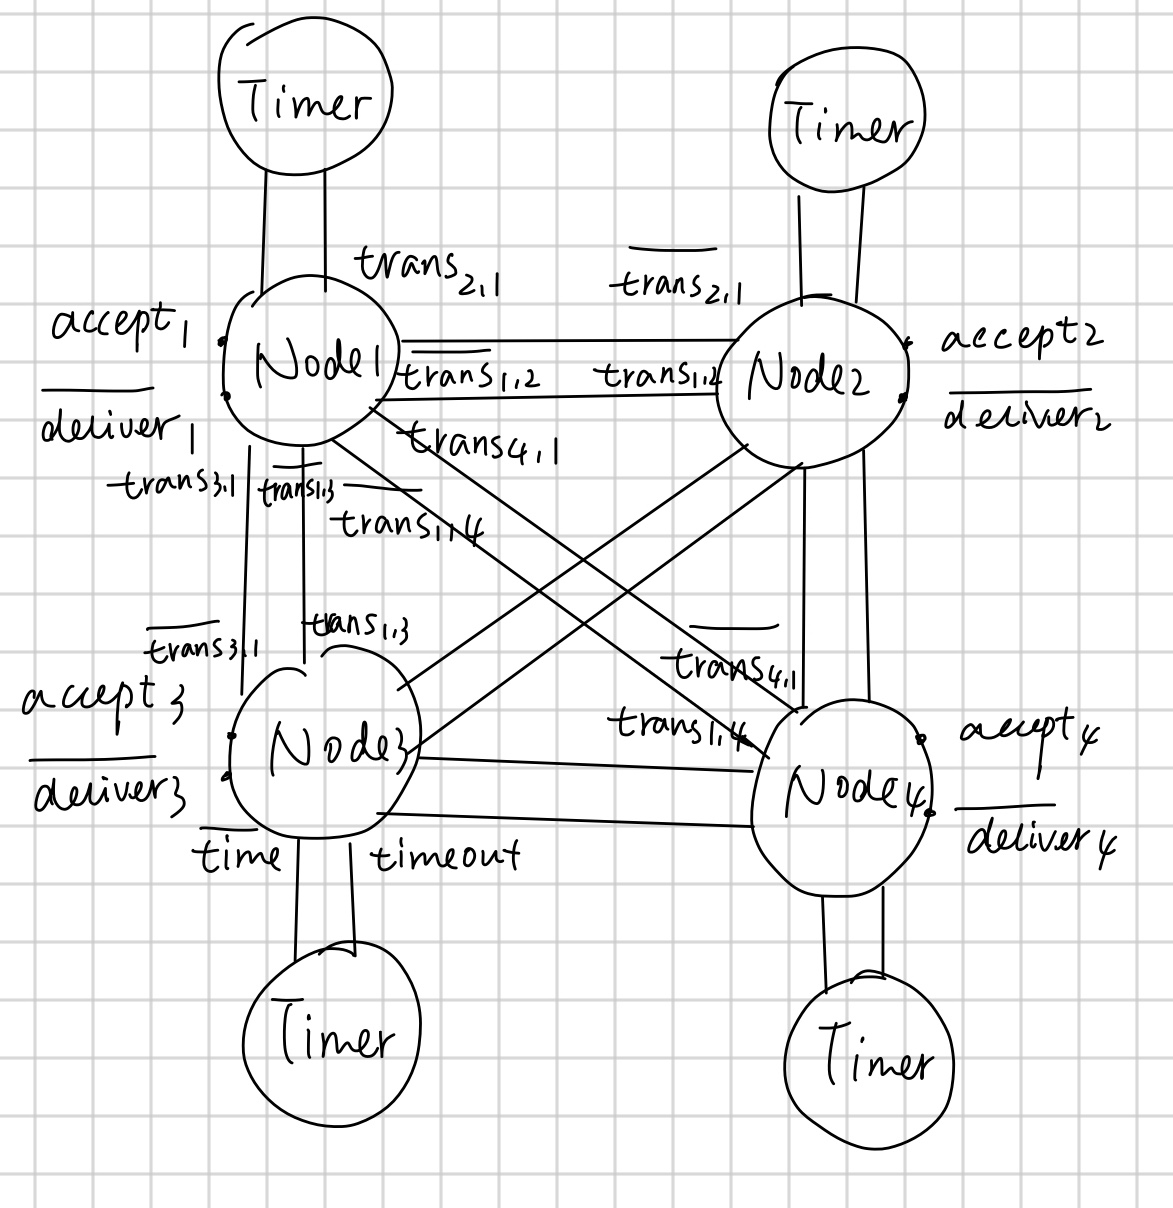
\includegraphics[width=11cm]{../figure/gossip2.jpg}
    \caption{\textbf{以Gossip协议作为通信协议的四节点的Peer-to-Peer Sysyem示意图}}
    \label{fig2}
\end{figure}

Gossip节点Node的状态有以下几种,分别对应Gossip协议中节点的状态:
\begin{table}[!hpt]
    \caption[节点状态对应]{节点状态对应\footnotemark}
    \label{tab:firstone}
    \centering
    \begin{tabular}{@{}llr@{}} \toprule
    %   \multicolumn{2}{c}{Item} \\ \cmidrule(r){1-2}
      节点状态 & Gossip状态 \\ \midrule
      Node&可接受系统外信息(除此状态外其余均不可接受外界信息)\\
      DeliveringNode&可向系统外传递信息\\
      UnInfectiousNode&未获取Gossip Message\\
      InfectiousNode&已获取Gossip Message\\
      GossipingNode&可向系统内部特定b个其他节点发送Gossip Message\\ \bottomrule
    \end{tabular}
  \end{table}

一个基于Gossip协议的Peer-to-Peer System的定义如下。
\begin{align*}
   Node_i& \stackrel{def}{=} accept_i(x).DeliveringNode_i(x)\\
   DeliveringNode_i(x) &\stackrel{def}{=} \overline{deliver_i}(x).InfectiousNode_i(x)\\
   InfectiousNode_i(x)&\stackrel{def}{=}timeout.(\bigoplus_{perm\in \mathsf{PERM}_i} p_{perm}\tau.GossipingNode_{i,perm}(x))\\
%    &+\sum_{j\in \mathsf{N}/\{i\}}trans_{j,i}(x).DeliveringNode_i(x)\\
   GossipingNode_{i,perm}(x)&\stackrel{def}{=}\overline{trans_{i,perm_{1}}}(x).\dots \overline{trans_{i,perm_{b}}}(x).\overline{time}.InfectiousNode_i(x)\\
   UnInfectiousNode_i &\stackrel{def}{=} \sum_{j\in \mathsf{N}/\{i\}}trans_{j,i}(x).DeliveringNode_i(x)\\
   GossipSystem_\mathsf{N}&\stackrel{def}{=}(Node_1\mid UnInfectiousNode_2\mid \dots \mid UnInfectiousNode_n)\\
   &\backslash \{trans_{i,j}\mid i\in \mathsf{N} \wedge j\in \mathsf{N} \wedge i\neq j\}\cup \{time, timeout\}
\end{align*}
在这个p2p-system中共有$n$个节点,标号为$\mathsf{N}$,每一个拥有gossip message的节点周期性的向$\mathsf{k}(\mathsf{k}\leq n-1)$个其他节点发送gossip message。
其中$\mathsf{PERM}_i$为$\mathsf{N}/\{i\}$中任选$\mathsf{k}$个元素的全排列。
上述定义基于一系列理想条件的假设:
\begin{itemize}
   \item [(1)] {网络传输可靠。然而现实中的网络传输存在丢包、延迟、比特反转等问题,
   我们可以通过ACK机制来解决[此处应有引用]。对不可靠网络下的Gossip协议,我们在上述理想条件下增加对网络传输的过程的建模,建模过程在Milner的CCS中有提及[此处应有引用]。}
   \item [(2)] {节点不会损坏。在现实中节点(也就是主机),是有寿命的,即在运行了一定时间后主机就会宕机,对于多个节点构成的p2p系统,存在节点失效的概率只会更高[此处应有引用:可参照MTTF],在后文对Membership的建模过程中我们会增加对这个问题的解决方案。}
   \item [(3)] {系统中只存在一个消息的传输。对于单个消息源的多个消息,我们仍然可以看作单个Gossip Message一起发送;对于多个消息源,我们可以为每个节点提供消息队列机制,来保存多个消息。
   在后续的Membership建模过程中还会提到。}
\end{itemize}

为了方便建模,我们假设一个节点选择任意其他节点作为Gossip的目标节点的概率是相同的,
即$p_{perm} = \frac{1}{A_{n-1}^{\mathsf{k}}} = \frac{(n-\mathsf{k}-1)!}{(n-1)!}$为固定值,当$\mathsf{k}=2$时,$p_{perm} = \frac{1}{(n-1)(n-2)}$。

\subsection{Push Gossip协议的等价性}

Gossip协议的目的是为了在系统内对节点进行多播,我们可以定义一个多播的Specification,同样我们只关注一个消息的多播:
\begin{definition} 
\begin{align*}
    MulticastSpec_\mathsf{N}&\stackrel{def}{=}accept_1(x).\overline{deliver_1}(x).Multicast_{\mathsf{N},\{1\}}(x)\\
    Multicast_{\mathsf{N},\mathsf{KNOWN}}(x)&\stackrel{def}{=}\tau.Multicasting_{\mathsf{N},\mathsf{KNOWN}}(x)\\
    Multicasting_{\mathsf{N},\mathsf{KNOWN}}(x)&\stackrel{def}{=}\overline{deliver_i}(x).Multicast_{\mathsf{N},\mathsf{KNOWN}\cup\{i\}}(x), \\
    &i\in \mathsf{N}-\mathsf{KNOWN} \wedge |\mathsf{N}|\neq |\mathsf{KNOWN}|
 \end{align*}
\end{definition} 

 \begin{definition} 
    \begin{align*}
   &GossipSystem_{\mathsf{N},(a,b,c)}(x)\\
   &= (\stackrel{a}{\overbrace{InfectiousNode(x)\mid \dots \mid InfectiousNode(x)}}\\
   &\mid \stackrel{b}{\overbrace{DeliveringNode(x)\mid \dots\mid DeliveringNode(x)}}\\
   &\mid \stackrel{c}{\overbrace{UnInfectiousNode\mid \dots \mid UnInfectiousNode}})\\
   &\backslash \{trans_{i,j}\mid i\in \mathsf{N} \wedge j\in \mathsf{N} \wedge i\neq j\}\cup \{time, timeout\}
\end{align*}
 \end{definition} 

\begin{theorem}
    $GossipSystem_{\mathsf{N}} \approxeq^s_{\mathsf{Th}} MulticastSpec_{\mathsf{N}}$,当$\top \in \mathsf{Th}$时成立。
\end{theorem}
\begin{proof}
每一个节点能且仅能执行一次deliver操作,且deliver的顺序不影响功能,
所以我们可以规定$A\stackrel{\overline{deliver_i}(t_1)}{\longrightarrow}_{\top} B$和$C\stackrel{\overline{deliver_j}(t_2)}{\longrightarrow}_{\top}B$是互模拟的当且仅当$t_1=t_2$,对下标是否一致不作要求。
因此在后文的证明中忽略了下标。

我们可以通过构建等价集,并证明等价集是一个symbolic bisimulation关系,来证明$GossipSystem_{\mathsf{N}} \approxeq^s_{\mathsf{Th}} MulticastSpec_{\mathsf{N}}$。

构造等价集
\begin{align*}
   \mathcal{S}&=\{(GossipSystem_{\mathsf{N}}, MulticastSpec_{\mathsf{N}}), \\
      &(GossipSystem_{\mathsf{N},(n,0,0)}(x), Multicasting_{\mathsf{N},\mathsf{N}}(x))\}\\
      & \cup \{(GossipSystem_{\mathsf{N},(a,b,c)}(x), Multicasting_{\mathsf{N}, \mathsf{KNOWN}}(x))\mid |\mathsf{KNOWN}| = a \wedge b\neq 0\}\\
      &\cup \{(GossipSystem_{\mathsf{N},(a,b,c)}(x), Multicast_{\mathsf{N}, \mathsf{KNOWN}}(x))\mid |\mathsf{KNOWN}| = a \wedge b= 0\}
\end{align*}

我们来依次证明$\mathcal{S}$中的每一对等价关系为symbolic bisimulation:
\begin{itemize}
    \item {
       $GossipSystem_{\mathsf{N},(n,0,0)}(x)$和$Multicasting_{\mathsf{N},\mathsf{N}}(x)$的$\top \mathcal{S}$-tree分别只有一个根节点,
       且不能转移至其他等价集,他们的互模拟性是显然的,实际上$GossipSystem_{\mathsf{N},(n,0,0)}(x)=Multicasting_{\mathsf{N},\mathsf{N}}(x)=0$。
    }
    \item {
        对于$(GossipSystem_{\mathsf{N},(a,b,c)}(x), Multicasting_{\mathsf{N}, \mathsf{KNOWN}}(x))\mid |\mathsf{KNOWN}| = a \wedge b\neq 0$:

        $GossipSystem_{\mathsf{N},(a,b,c)}(x)$的$\top \mathcal{S}$-tree $t$如图所示:

        对$t$的叶子结点有$L\stackrel{\overline{deliver}(x)}{\longrightarrow}_{\top} GossipSystem_{\mathsf{N},(a+1,b-1,c)}(x)$。
        即
        
        $(GossipSystem_{\mathsf{N},(a,b,c)}(x)\rightsquigarrow_{\top\mathcal{S}}\stackrel{\overline{deliver}(x)}{\longrightarrow}_{\top}[GossipSystem_{\mathsf{N},(a+1,b',c')}(x)]_{\top\mathcal{S}},b'+c'=b+c-1$。

        % 对应的$Multicasting_{\mathsf{N}, \mathsf{KNOWN}}(x)\rightsquigarrow_{\top\mathcal{S}}\stackrel{\overline{deliver}(x)}{\longrightarrow}_{\top\mathcal{S}} []$
        \begin{itemize}
            \item {\textbf{Case 1. $b>1$}}
            \item {\textbf{Case 2. $b=1$}}
        \end{itemize}
    }
    \item {
        对于$(GossipSystem_{\mathsf{N},(a,b,c)}(x), Multicast_{\mathsf{N}, \mathsf{KNOWN}}(x))\mid |\mathsf{KNOWN}| = a < n \wedge b= 0$:

        $Multicast_{\mathsf{N}, \mathsf{KNOWN}}(x)$的$\top \mathcal{S}$-tree只有一个根节点,
        且有$Multicast_{\mathsf{N}, \mathsf{KNOWN}}\rightsquigarrow_{\top\mathcal{S}}\stackrel{1}{\rightarrow}_{\top}[Multicasting_{\mathsf{N}, \mathsf{KNOWN}}]_{\top \mathcal{S}}$。

        $GossipSystem_{\mathsf{N},(a,b,c)}(x)$的$\epsilon$-tree $t$如图所示:

        $GossipSystem_{\mathsf{N},(a,b,c)}(x)$的$\top\mathcal{S}$-tree $t'$为:
        $GossipSystem_{\mathsf{N},(a,b,c)}(x)\stackrel{(\top,p')}{\rightarrow}GossipSystem_{\mathsf{N},(a,b,c)}(x)\stackrel{(\top,p')}{\rightarrow}\cdots$,
        其中$p'= (\frac{A^k_{a-1}}{A^k_{n-1}})^a = (\frac{(a-1)!}{(n-1)!})^a = O(\frac{1}{n})<1$。
        $\mathsf{P}^f(t) = 1-\lim_{level\rightarrow \infty} (p')^{level} = 1$,则$GossipSystem_{\mathsf{N},(a,b,c)}(x)$的$\epsilon$-tree $t$为regular tree,
        且$\mathsf{P}^f(t) = \sum \{p_i\mid L_i\stackrel{p_i\tau}{\rightarrow} [GossipSystem_{\mathsf{N},(a,b',c')}(x)]_{\top \mathcal{S}}\}$,
        其中$b'>0 \wedge b'+c'=b+c$,
        则
        $$GossipSystem_{\mathsf{N},(a,b,c)}(x)\rightsquigarrow_{\top\mathcal{S}}\stackrel{1}{\rightarrow}_{\top}[GossipSystem_{\mathsf{N},(a,b',c')}(x)]_{\top \mathcal{S}}$$
    }
    \item {
        余下的一组证明是常规的VPC证明。
    }
 \end{itemize}

\end{proof}
\subsection{Gossip Style Membership的实现}

\section{Gossip Style Membership的仿真模拟}